\begin{figure}[t]
    \centering
    \setlength{\resLen}{1in}
    \addtolength{\tabcolsep}{-3pt}
    \small
    \begin{tabular}{ccc}
        & Forward & Backward\\
        \includegraphics[height=.9\resLen]{particle/aniso_z.png}
        & \multicolumn{2}{c}{\includegraphics[height=\resLen]{pfunc/aniso_z.png}}
        \\
        \includegraphics[height=.9\resLen]{particle/aniso_y.png}
        & \multicolumn{2}{c}{\includegraphics[height=\resLen]{pfunc/aniso_y.png}}
        \\
        \textbf{(a) Incident direction} & \multicolumn{2}{c}{\textbf{(b) Phase function slice}}
    \end{tabular}
    \caption{\label{fig:aniso1}
        Visualizations of slices $\phase(\dwi,\cdot)$ of a phase function for two incident directions~$\dwi$ at $\lambda = 700\text{nm}$.
        This phase function is computed using a configuration where 100 particles with radii 300nm follow an anisotropic Gaussian distribution.
    }
\end{figure}
